
In this section, we propose a unified computational account of \emph{ad hoc} coordination and convention formation that addresses these three empirical puzzles. 
We begin from first principles: What is the core computational problem that must be solved to achieve successful communication?
Classically, this problem has been formulated in terms of coding and compression \cite{Shannon48}. 
An intended meaning in the speaker's mind must be encoded as a signal that is recoverable by the receiver after passing through a noisy transmission channel.
This literal transmission problem has since been enriched to account for \emph{pragmatics} -- the ability of speakers and listeners to use context and social knowledge to draw inferences beyond the literal meaning of messages \cite{sperber1986relevance}.
We take the Rational Speech Act framework \cite<RSA;>{frank_predicting_2012,goodman_pragmatic_2016,FrankeJager16_ProbabilisticPragmatics} as representative of this current synthesis, formalizing communication as recursive social inference in a probabilistic model.
In the next section, we will review this basic framework and then raise two fundamental computational problems facing this framework that motivate our proposal.

\subsection{RSA models of communication with static meaning}

In our referential communication setting\footnote{For concreteness, we restrict our scope to reference in a discrete context of objects, but the same formulation applies to more general spaces of meanings.}, the RSA framework defines a pragmatic speaker, denoted by $S_1$, who must choose an utterance $u$ that will allow their partner to choose a particular target object $o$ from the current communicative context $\mathcal{C}$:
They attempt to satisfy the Gricean Maxims \cite{Grice75_LogicConversation} by selecting utterances proportional to a utility function $U(u;o)$ that balances informativity to an imagined listener against the cost of producing an utterance:
\begin{align}
S_1(u | o) & \propto   \exp\{w_S \cdot U(u; o)\}\label{eq:RSAspeaker} \\
U(u; o) & = (1-w_C) \cdot \underbrace{\log L_0(o | u)}_{\mathclap{\text{informativity}}} -\, w_C \cdot \underbrace{c(u)}_{\mathclap{\text{cost}}} \nonumber 
\end{align}
where $c(u)$ is a function giving the cost of producing $u$, assuming a longer utterances are more costly.
The speaker has two free parameters: $w_C \in [0,1]$ controls the relative weight of informativity and parsimony in the speaker's production, and $w_S \in[0,\infty]$ controls their softmax optimality (i.e. as $w_S \rightarrow \infty$, the speaker increasingly chooses the utterance with maximal utility.)

The imagined \emph{literal listener} $L_0$ in Eq.~\ref{eq:RSAspeaker} is assumed to identify the target using a lexical meaning function $\mathcal{L}(u,o)$ capturing the literal semantics of the utterance $u$.
That is, the probability of the literal listener choosing object $o$ is proportional to the meaning of $u$ under a static function $\mathcal{L}$:
\begin{align}
L_0(o | u) &\propto  \mathcal{L}(u,o)\hfill\label{eq:RSA}
\end{align}
Throughout this paper, we will take $\mathcal{L}$ to be a traditional truth-conditional function evaluating whether a given object is in the extension of the utterance\footnote{Note that the normalization constant may be exactly zero for some possible lexicons -- for instance, if a given utterance is literally false of all objects in context -- in which case these distributions are not well-defined. See Appendix A for full details of how we address this problem.}:
$$\mathcal{L}(o,u) = \left\{ \begin{array} {rl} 1 & \textrm{if $o \in $\den{u}} \\ 0 & \textrm{otherwise} \end{array}\right.$$
However, this formulation is also consistent with fuzzier, continuous semantics \cite{degen2020redundancy} as may be learned by a (grounded) neural network \cite[see Appendix B for an example]{potts2019case}.

Finally, we may then define a pragmatic listener $L_1$ that inverts an internal model of the speaker to infer which intended referent $o\in\mathcal{C}$ would best explain the speaker's choice of utterance $u$:
\begin{align}
L_1(o | u) \propto   \exp\{w_L \cdot \log S_1(u | o)\}
\end{align}
where $w_L \in[0,\infty]$ controls the listener's soft-max optimality.
Intuitively, this listener considers whether a speaker trying to refer to different objects $o$ would be likely to produce utterance $u$, accounting for the alternative utterances the speaker could have produced. 

\subsection{Fundamental problems for static meaning}

This basic framework and its extensions have accounted for a variety of important phenomena in pragmatic language use \cite<e.g.>{Scontras_problang,KaoWuBergenGoodman14_NonliteralNumberWords,TesslerGoodman16_Generics,LassiterGoodman15_AdjectivalVagueness}.
Yet it retains a key assumption from classical models: that the speaker and listener must share the same literal ``protocol'' $\mathcal{L}$ for encoding and decoding messages.
In this section, we highlight two under-appreciated challenges of communication that complicate this assumption. 

The first challenge is \emph{variability} in linguistic meaning throughout a language community. 
Different listeners may recover systematically different meanings from the same message, and different speakers may encode the same message in different ways.
For example, doctors may fluently communicate with one another about medical conditions using specialized terminology that is meaningless to a patient. 
The words may not be in the patient's lexicon, and even common words may be used in non-standard ways.
That is, being fluent speakers of the same language does not ensure perfect overlap for the relevant meanings that need to be transmitted in every context: different partners may simply be using different functions $\mathcal{L}$.

The second challenge is the \emph{non-stationarity} of the world. 
Agents are continually presented with new thoughts, feelings, and entities, which they may not already have efficient conventions to talk about.
For example, when new technology is developed, the community of developers and early adopters must find ways of referring to the new concepts they are working on (e.g. \emph{e-mailing}, \emph{the Internet}). 
Or, when researchers design a new experiment with multiple conditions, they must find ways of talking about their own \emph{ad hoc} abstractions, often converging on idiosyncratic names that can be used seamlessly in meetings.
That is, any literal protocol $\mathcal{L}$ that we may write down at one time would be quickly outdated at a later time \cite<see>[for a demonstration of the related problems posed by non-stationary for large neural language models]{lazaridou2021pitfalls}.
We must have some ability to extend our language on the fly as needed.

\subsection{A hierarchical model of dynamic meaning}

%The model we present in this section aims to provide an explanation for how agents may  these fundamental problems.
Rather than assuming a monolithic, universally shared language, we argue that agents solve the core problems posed by variability and non-stationarity by attempting to continually, adaptively \emph{infer} the system of meaning used by their partner in context.
When all agents are continually learning in this way, we will show that they are not only able to locally coordinate with specific partners but also able to abstract away shared linguistic conventions.
We introduce our model in three steps, corresponding to three core capacities: uncertainty about meaning, online partner-specific learning, and inductive generalization.

\paragraph{Hierarchical uncertainty about meaning} 

When an agent encounters a communication partner, they must call upon some representation about what they expect different signals will mean to that partner. 
We therefore replace the static function $\mathcal{L}$ with a \emph{parameterized family} of lexical meaning functions by $\mathcal{L}_{\phi}$, where different values of $\phi$ yield different possible systems of meaning. 
While we will remain agnostic to the exact form of this function, and the space of $\phi$, there are two key computational desiderata we emphasize.
First, given the challenge of variability raised in the previous section, these expectations ought to be sensitive to the overall statistics of the population. 
An agent should know that there is tighter consensus about the meaning of \emph{dog} than the meaning of, say, specialized medical terms like \emph{sclerotic aorta} \cite{Clark98_CommunalLexicons}, and conversely, should expect more consensus around how to refer to familiar concepts than new or ambiguous concepts.
Second, this representation should also, in principle, be sensitive to the social identity of the partner: a cardiologist should have different expectations about a long-time colleague than a new patient.

The first desideratum, representing population variability, motivates a \emph{probabilistic} formulation.
Instead of holding a single static function $\mathcal{L}_{\phi}$, which an agent assumes is shared perfectly in common ground (i.e. one $\phi$ for the whole population), we assume each agent maintains \emph{uncertainty} over the exact meaning of words as used by different partners.
In a Bayesian framework, this uncertainty is specified by a prior probability distribution over possible values of $\phi$ \ks{I found this quite hard to interpret because phi is quite abstract at the moment}.
The introduction of uncertainty over a partner's literal semantics has previously been explored in the context of one-shot pragmatic reasoning, where it was termed \emph{lexical uncertainty} \cite{bergen_pragmatic_2016}, and in the context of iterated dyadic interactions \cite{SmithGoodmanFrank13_RecursivePragmaticReasoningNIPS}. 

The second desideratum, sensitivity to partner-specific meanings, motivates a \emph{hierarchical} model, where uncertainty is represented by a multi-level prior. 
At the highest level of the hierarchy is \emph{community-level} uncertainty $P(\Theta)$, where $\Theta$ represents an abstract ``overhypothesis" about the overall distribution of possible partners. 
$\Theta$ then parameterizes the agent's \emph{partner-specific} uncertainty $P(\phi_{k} | \Theta)$, where $\phi_k$ represents the specific system of meaning used by partner $k$ (see Fig. \ref{fig:model_schematic}). 
To integrate this uncertainty into our speaker and listener models, we assume they each act in a way that is expected to be successful \emph{on average}, under likely values of $\phi_k$.
In other words, they sample actions by marginalizing over the posterior $P(\phi_k | D_k)$ of different language models their partner may be using.
\begin{align}
L(o|u) &\propto   \exp\left\{w_L \textstyle{\int} P(\phi_k | D_k)  \log S_1(u|o, \phi_k)\,\,d\phi_k\right\}\label{eq:marginalized}\\
S(u|o) &\propto  \exp\left\{w_S \textstyle{\int} P(\phi_k | D_k)  U(u; o, \phi_k) \,\,d\phi_k\right\}\nonumber
\end{align}

\paragraph{Partner-specific learning}

\begin{figure}[t!]
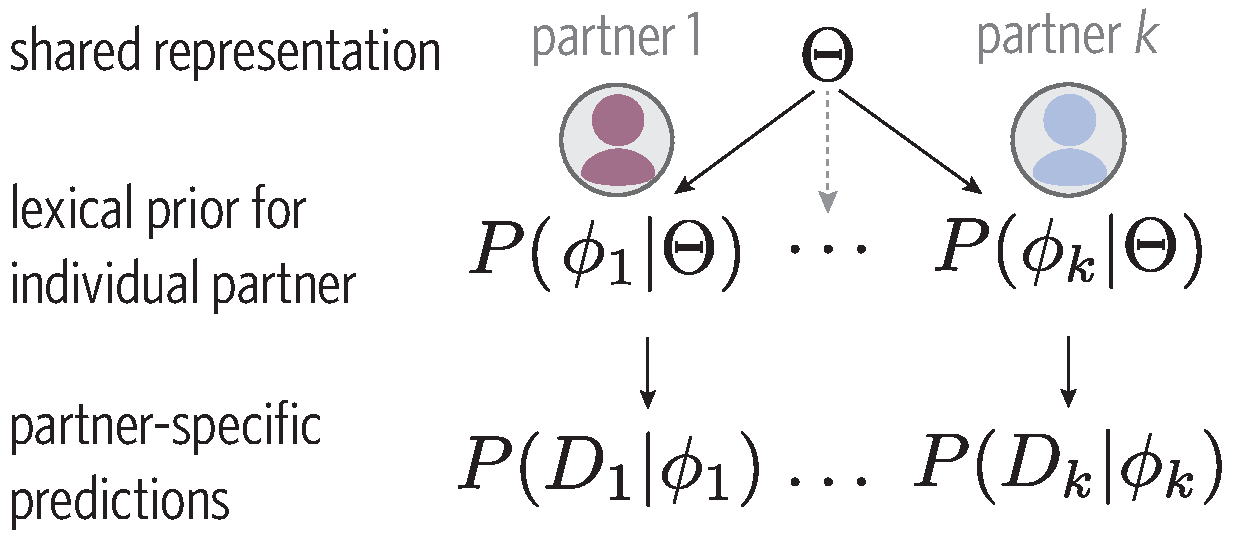
\includegraphics[scale=0.4]{./figures/task1_model.pdf}
\vspace{.5em}
\caption{\emph{Schematic of hierarchical Bayesian model.} At the highest level, denoted by $\Theta$, is a representation of aspects of meanings expected to be shared across all partners. These \emph{global} conventions serve as a prior for the systems of meanings used by specific partners, $\phi_k$. These partner-specific representations give rise in turn to predictions about their language use $P(D_k|\phi_k)$, where $D_k$ represents observations in a communicative interaction with partner $k$. By inverting this model, agents can adapt to \emph{local} partner-specific conventions and update their beliefs about global conventions.}
\label{fig:model_schematic}
\end{figure}

This formulation derives how agents ought to act given a certain set of partner-specific beliefs about $\phi_k$.
But where do these beliefs come from?
Although an agent may begin with significant uncertainty about the system of meaning their partner is using in the current context, an extended interaction provides useful information for reducing that uncertainty and therefore improving the success of communication.
In other words, \emph{ad hoc} convention formation may be re-cast as an inference problem.
Given observations $D_k$ from interactions with partner $k$, an agent can update their beliefs about their partner's latent system of meaning following Bayes rule:
\begin{equation}
\begin{array}{rcl}
\label{eq:joint_inference}
P(\phi_k, \Theta | D_k)  & \propto &  P(D_k | \phi_k, \Theta) P(\phi_k, \Theta) \\
                           & =   & P(D_k | \phi_k) P(\phi_k | \Theta) P(\Theta)
\end{array}
\end{equation}
This joint inference decomposes the learning problem into two terms, a prior term $P(\phi_k | \Theta)P(\Theta)$ and a likelihood term $P(D_k | \phi_k)$.
The prior term captures the idea that, in the absence of strong evidence of partner-specific language use, the agent ought to regularize toward their background knowledge of conventions: the aspects of meaning that all partners are expected to share in common.
The likelihood term represents predictions about how a partner would use language in context under different underlying systems of meaning (i.e. based on Eq.~\ref{eq:RSA}: see \emph{Referential Feedback} section below).

Importantly, this posterior allows agents to maintain partner-specific expectations about $\phi_k$, as used in Eq.~\ref{eq:marginalized}, by marginalizing over community-level uncertainty:
\begin{equation}
P(\phi_k | D_k) =  \int_{\Theta}P(\phi_k, \Theta | D_k)  d\Theta
\end{equation}
This posterior can be viewed as the ``idiolect'' that has been fine-tuned to account for partner-specific common ground from previous interactions.
We will show that when agents learn about their partner in this way, and adjust their own production or comprehension accordingly (i.e.~Eq.~\ref{eq:marginalized}), they are able to coordinate on stable \emph{ad hoc} conventions.

\ks{I had a crappy non-hierarchical model in this 2017 paper, basically comparing the two extremes you talk about later (complete pooling and no pooloing): http://dx.doi.org/10.1098/rstb.2016.0051} 

\paragraph{Inductive generalization}

The posterior in Eq.~\ref{eq:joint_inference} also provides an inductive pathway for partner-specific data to inform beliefs about community-wide conventions.
Agents update their beliefs about $\Theta$ by marginalizing over data accumulated from different partners:
\begin{equation}
\begin{split}
    P(\Theta | D)  = & \int_{\phi} P(\phi_k, \Theta | D_k) d\phi \\
%                     \propto & P(\Theta) \int_{\phi} P(D_k | \phi_k) P(\phi_k | \Theta) d\phi
\end{split}
\end{equation}
where $D = \bigcup_{k=1}^N D_k$, $\phi = \phi_1 \times \dots \times \phi_N$, and $N$ is the number of partners previous encountered. 
Intuitively, when multiple partners are inferred to use similar systems of meaning, beliefs about $\Theta$ shift to represent this abstracted knowledge: it becomes more likely that a novel partner in one's community will share it as well.
In other words, this updated $\Theta$ should be used to guide the prior expectations an agent brings into a subsequent interactions with a stranger.
This transfer is sometimes referred to as ``sharing of strength'' or ``partial pooling'' because pooled data is smoothly integrated with domain-specific knowledge.
This property has been key to explaining how the human mind solves a range of other difficult inductive problems in the domains of concept learning \cite{KempPerforsTenenbaum07_HBM, tenenbaum_how_2011}, causal learning \cite{KempGoodmanTenenbaum10_LearningToLearn,GoodmanUllmanTenenbaum11_TheoryOfCausality},  motor control \cite{berniker2008estimating}, and speech perception \cite{kleinschmidt2015robust}.

\subsection{Further challenges}

The formulation in the previous section presents the core of our theory.
Here, we highlight several additional features of our model, which address more specific challenges raised by prior work on communication and which we will encounter in the simulations reported in the remainder of the paper. 
Our organization of these details is motivated by \citeA{spike_minimal_2017}, which recently distilled three common problems that all accounts of convention must address: (1) the availability of referential feedback, (2) a form of information loss or forgetting, and (3) a systemic bias against ambiguity.
Finally, we will explain (4) the more practical details of how we perform inference in this model. 

\paragraph{Referential feedback}

Learning and adaptation depends on the availability and quality of observations $D_k$ throughout a communicative interaction.
If the speaker has no way of assessing the listener's understanding, or if the listener has no way of comparing their interpretation against the speakers intentions, however indirectly, they can only continue to rely on their prior, with no ground for conventions to form  \cite{KraussWeinheimer66_Tangrams,HupetChantraine92_CollaborationOrRepitition,GarrodFayLeeOberlanderMacLeod07_GraphicalSymbolSystems}.
So, what data $D_k$ should each agent use to update their beliefs at a particular point in an interaction?

In principle, we expect that $D_k$ reflects all relevant sources of information that may expose an agent's understanding or misunderstanding, including verbal and non-verbal backchannels (\emph{mmhmm}, nodding), clarification questions, and actions in the world.
In the narrower setting of a reference game, we consider the full referential feedback provided by the task: $D_k = \{(o^*, u, o')\}_{t=1}^T$, where $o^*$ denotes the speaker's intended target, $u$ denotes the utterance they produced, $o'$ denotes the listener's response.
In particular, agents should condition on feedback from their \emph{partner's} choices.
The listener should use the probability that their partner would produce $u$ to refer to the target $o^*$ under different $\phi_k$, and the speaker should likewise use the probability that their partner would produce response $o'$ after hearing utterance $u$.

This symmetrical relationship, where each agent is learning from the other's behavior, creates a clear coordination problem.
In the case of an error, where the agent in the listener role hears the utterance $u$ and chooses an object $o'$ other than the intended target $o^*$, they will receive feedback about the intended target and subsequently condition on the fact that the speaker chose $u$ to convey that target, $P_S(u | o^*)$. \ks{Worth pointing out that you are assuming that the speaker's target and the listener's response are at some point manifest to both?}
\ks{I also realised just now that you are using modality-specific terminology of "speaker" and "listener" - there are no good modality-neutral terms that I have seen, but just to flag up that people working on sign find this annoying.}
Meanwhile, the agent in the speaker role will subsequently condition on the likelihood that the listener chose the object $o'$ upon hearing their utterance $P_L(o' | u)$.
In other words, each agent will subsequently condition on slightly different data\footnote{In some settings, agents in one role may be expected to take on more of the burden of adaptation, leading to an asymmetric division of labor \cite<e.g.>{MorenoBaggio14_AsymmetrySignaling}. This may be especially relevant in the presence of asymmetries in power, status, or capability. We leave consideration of these asymmetries for future work.}.

\paragraph{Memory and forgetting}

Second, we must address the limitations imposed by memory and forgetting; it is unrealistic to expect that memories of every element of every past interaction in $D$ is equally available.
%Some \emph{forgetting} or \emph{discounting} mechanism appears necessary for convention formation. 
Furthermore, this may be to the agent's advantage. 
As described in the previous section, early errors are incorporated into the data, leading to mis-coordination much later in an interaction when each agent conditions on different data.
Without a mechanism to discount these earlier data points, agents may be prevented from ever reaching consensus \cite{spike_minimal_2017}.

Forgetting is typically incorporated into Bayesian models with a decay term in the likelihood function \cite{anderson2000adaptive,angela2009sequential,fudenberg2014recency,kalm2018visual}.
$$P(D_k | \phi_k) = \prod_{\tau=0}^t \beta^{t-\tau} P(\{o,u\}_\tau | \phi_k)$$
This decay is motivated by the empirical power function of forgetting \cite{wixted1991form}, and can be interpreted as the expectation over a process where observations have some probability of dropping out of memory at each time step.
Alternatively, at the algorithmic level, decay can be viewed as a form of weighted importance sampling, where more recent observations are preferentially sampled \cite{pearl2010online}.

\paragraph{Bias against ambiguity}

A third specific challenge is posed by potential ambiguity about \emph{ad hoc} conventions.
If a speaker uses an expression to refer to one particular target, it is consistent with that data to believe that the same expression is perfectly acceptable for the other targets as well. 
%How do agents overcome this ambiguity to converge on an \emph{informative} communication system?
In our account, this problem is naturally solved by the principles of \textit{pragmatic reasoning} \cite{Grice75_LogicConversation}.
Pragmatic reasoning plays two distinct roles in our model.
First, Gricean agents must assume that their partner is using language in a cooperative manner and account for this when inferring their partner's language model.
That is, we use these equations as the linking function in the likelihood $P(D_k | \phi_k)$, representing an agent's prediction about how a partner with meaning function $\phi_k$ would actually behave in context (Eq.~\ref{eq:joint_inference}). 
$S_1$ is used to learn from observations generated in the speaker role and $L_1$ is used to learn from observations generated in the listener role.
Second, agents do not only make passive inferences from observation, they participate in the interaction by \emph{using language} themselves.
A Gricean agent's own production and comprehension is also guided by cooperative principles (Eq.~\ref{eq:marginalized}).

Many minor variations on the basic RSA model have been explored in previous work, and it is worth highlighting two technical choices in our formulation.
First, in the likelihoods given in Eq.~\ref{eq:RSA}, both agents use an ``action-oriented'' representation to update their beliefs about their partner, in the sense that their partner is expected to behave proportional to the utility of different actions, according to a soft-max normalization $\sigma(U(z)) = e^{U(z)}/\sum e^{U(z)}$.
This contrasts with some RSA models outside the scope of reference games, where the listener is instead assumed to be ``belief-oriented,'' simply inferring the speaker's intended meaning without producing any action of their own \cite{qing2015variations}.
Additionally, as their decision rule, agents sample actions proportion to their own soft-max distribution (Eq.~\ref{eq:marginalized}).
That is, while it is possible for agents to use a soft-max likelihood to predict their partner's behavior but \emph{maximize} their own utility when taking action, we have agents use the same soft-max distribution in both cases.
See Appendix for further details about the definition and implementation of the RSA likelihood.

\paragraph{Inference details}

While our simulations in the remainder of the paper each address different scenarios, we have aimed to hold as many details as possible constant throughout the paper.
First, we must first say what functional representation we are using for the agents' lexicon $\mathcal{L}_{\phi}$.
For consistency with previous Bayesian models of word learning \cite<e.g.>{XuTenenbaum07_WordLearningBayesian} we have chosen to represent the space of meanings for an utterance as the set of nodes in a concept taxonomy\footnote{Note there are many alternative representational choices compatible with our core model, including parameterized vector embeddings and multi-layer neural networks, which may be more appropriate for scaling our model to larger spaces of words and referents. We return to these possibilities in the General Discussion.}.
When targets of reference are conceptually distinct, as assumed in most prior models of signaling games, the taxonomy is flat and the target space of utterance meanings reduces to the space of individual objects, i.e.~$\den{u}_{\phi} = \phi(u) \in \mathcal{O}$ for all $u\in\mathcal{U}$, where different values of $\phi$ correspond to different mappings between utterances and objects \ks{again, might need to unpack this a bit}. 
However, in our simulations for \textbf{P3}, we will also consider sets of referents with more complex  conceptual structure, and more abstract meanings applying to multiple referents.
To cover all of these cases, the lexical meaning function is defined to be
$$
\mathcal{L}_\phi(o,u) = \left\{ \begin{array} {rl} 1 & \textrm{if $o \in \phi(u)$} \\ 0 & \textrm{otherwise} \end{array}\right.
$$
\ks{and more explanation needed here}
We then assume a simplicity prior over possible lexicons, $P(\phi) \propto \exp\{|\phi|\}$, where $|\phi|$ is the total size of each word's extension, summed across words in the vocabulary \cite{FrankGoodmanTenenbaum09_Wurwur}. \ks{If I am reading it right, this isn't actually what I was expecting the simplicity prior to be - are you favouring small word meanings, rather than small numbers of words? Seems potentially contentious to me, I would go absolutely the opposite direction!}

We have implemented all of our simulations in the probabilistic programming language WebPPL \cite{GoodmanStuhlmuller14_DIPPL}, and have made them available online along with materials for reproducing our experiments and analyses\footnote{\url{github.com/hawkrobe/conventions_model}}.
In all cases, we run our simulations by iterating the following trial-level loop: (1) sample an utterance from the speaker's utterance distribution, given the target object, (2) sample an utterance\ks{should be object?} from the listener's object distribution, given the utterance sampled in the previous step, (3) append the results to the list of observations, and (4) update both agents' posterior distributions, conditioning on these observations before continuing to the next trial.

To obtain the speaker and listener distributions (steps 1-2; Eq.~\ref{eq:RSA}), we use enumeration for exact inference.
We would also prefer to use enumeration to obtain posteriors over lexical meaning (step 4; Eq.~\ref{eq:joint_inference}), but as the space of possible lexicons $\phi$ grows, this approach becomes intractable.
For simulations related to \textbf{P2} and \textbf{P3}, we therefore switch to Markov Chain Monte Carlo (MCMC) methods to obtain samples from the posterior, and take the expectations in Eq.~\ref{eq:marginalized} as a sum over these samples. 
Finally, because we are emphasizing a set of phenomena where our model makes qualitatively different predictions than previous models, our goal in this paper is to illustrate and evaluate these \emph{qualitative} predictions rather than provide exact quantitative fits to empirical data.
As such, we will proceed by deriving predictions for a regime of parameter values ($w_S, w_L, w_C,\beta$) that make the strongest predictions, and leave the identification of the best-fitting parameters for future work. 
